\documentclass[conference,letterpaper,twocolumn]{IEEEtran}

%\usepackage[ansinew]{inputenc}
\usepackage{graphicx}
\usepackage{psfrag}
\usepackage{stfloats}
%\usepackage[spanish]{babel}
\usepackage{epsfig}
\usepackage{pifont}
\usepackage{amssymb}
\usepackage{fixltx2e}
\usepackage{amsmath}
\usepackage{rotate}
\usepackage{anysize}
%\usepackage{rotating}
%\usepackage{fancybox}
\usepackage{float}
\usepackage{fancybox}
\usepackage{subfig}

\newcommand{\pig}[1]{\mbox{\boldmath ${#1}$}	}

\newtheorem{Theod}{{\bf Definici\'on}}

\setlength{\oddsidemargin}{-5mm}
\setlength{\evensidemargin}{5mm}
\setlength{\topmargin}{-3mm}
\setlength{\textwidth}{17cm}
\setlength{\columnsep}{5mm}
\setlength{\textheight}{25cm}

\begin{document}

\title{Double bounded polynomial homotopy applied to non-linear circuit simulation}



\maketitle

\begin{abstract}

This work shows a new double bounded Homotopy based on polynomial formulation. It presents a bounding between two solution lines and a symmetry axis,which allows to establish a stop criterion for the simulation. Besides, the initial and final points for the new double bounded Homotopy may be established in an arbitrary manner. Mathematical properties will be introduced for this new Homotopy, besides, some mathematical and circuital examples will be discussed.

\end{abstract}
 

\section{Introduction}

The problem to find solutions in DC is important because this analysis serves as initial point for the rest of analysis performed routinely during the circuit design (for instance, small signal analysis)\cite{homo_ogrodzki}. This analysis consists in finding solutions for non-linear algebraic equations system (NAEs) originating from integrated circuits \cite{Schwa_book}. These NAEs become complex because the accelerated increase on the number of transistors by ICs and the increase of complexity of models (as the result of reducing the physical dimensions of the components) causing two situations: existence for multiple unexpected operating points, and lack of convergence to the operating point in Newton's method.

The Newton-Raphson method (NR) is employed in many circuit simulators for integrated circuit. Nevertheless, the NR method has certain convergence problems \cite{Schwa_book} like: oscillation and divergence. This situation has prompted investigations to develop new methods capable to solve non-linear equation systems in an efficient and accurate process.
Homotopy methods \cite{BHLHOM,homo_ArtificialP} are valuable tools for simulation, presented as an alternate method to the NR method. However, Homotopy methods does not have stop criterion. Hence, the Double bounded polynomial Homotopy is introduced in this work in order to circumvent the problem of stop criterion.


\section{Double bounded polynomial Homotopy}

The double bounded polynomial Homotopy (DBP) is defined by the following equation:

\begin{equation}
{\small
\begin{array}{l}
H(f(x)),\lambda )=Q(x-x_i)(x-x_f) -C(\lambda-a/2)^2 f(x)^2
\end{array}}
\label{homotopiaP}
\end{equation}

where $Q=\lambda(\lambda-a)$, $a$ is a constant that represents the separation between solution lines, $x_i$ is the initial point, $x_f$ the final point, and $C$ an arbitrary constant.

Based on the preceding, Homotopy can be expressed in general way as:

\begin{displaymath}
\pig{H}(\pig{f}(\pig{x}),\lambda ) = \left\{\begin{array}{rl}
f(x^*)=0 & \textrm{para $\lambda=0$ y $x=x^*$}\\
P=0 & \textrm{para $\lambda=a/2$}\\
f(x^*)=0 & \textrm{para $\lambda=a$ y $x=x^*$}
\end{array}\right.
\end{displaymath}

where $P=(x-x_i)(x-x_f)$, $x^*$ is any solution for the equilibrium equation $f(x)$, $x_i$ in the initial point, while $x_f$ is the final point for outline the path.

This Homotopy has two solution lines ($\lambda=0$ y $\lambda=a$). Squaring function $f(x)$ originates an even number of solutions (or operating points) resulting in the bounding of it and closes the Homotopy path within the middle region. Figure \ref{halftrack} shows how the Homotopy path initiates at $A=(x_i,a/2)$ on the symmetry axis, finds two roots (in region $\lambda_2(x)$) and, finally, ends when a new crossing the symmetry axis at $B=(x_f,a/2)$ meaning that the tracing of a symmetrical branch is completed fulfilling the stop criterion.

\begin{figure}[hbtp]
\psfrag{o}{$\lambda$}
\psfrag{a}[][][0.7]{$\lambda_1$}
\psfrag{b}[][][0.7]{$\lambda_2$}
\psfrag{c}[][][0.7]{$\lambda_{sym}=a/2$}
\centering
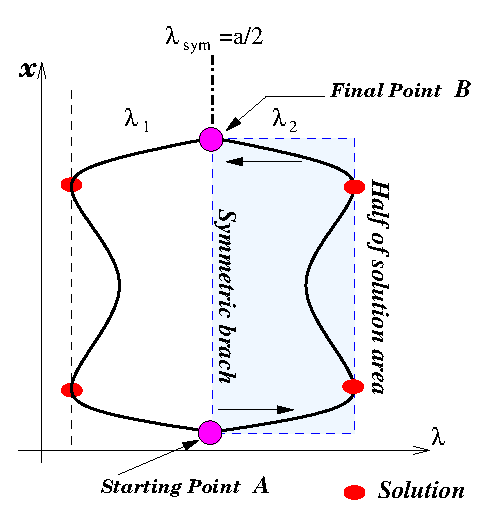
\includegraphics[scale=0.55]{fig/dbh2.eps}
\caption{Stop criterion.}
\label{halftrack}
\end{figure}

Properties of this new Homotopy are presented in the following sub-sections:

\subsection{Symmetrical branches}

Symmetrical branches shown in figure \ref{halftrack} can be obtained solving for $\lambda$ equation \ref{homotopiaP}. The result is two symmetrical branches (ecuaciones \ref{SB1} y \ref{SB2}), where each symmetrical branch $\lambda_1(x)$ and $\lambda_2(x)$is tied to a different solution line $\lambda=0$ and $\lambda=a$, respectively. Given that $\lambda_1(x)$ and $\lambda_2(x)$ are connected and symmetrical, it is just necessary to trace only one of them to obtain the complete path and finish the simulation. $\lambda_2(x)$ is chosen as the path to trace, it touches tangentially solution line $\lambda=a$.

\begin{equation}
\lambda_1(x)= {\frac {\left( \sqrt {1-{\frac {C \left( f \left( x \right)  \right) ^{2
}}{ \left( x-x_i \right)  \left( x-x_f \right) }}}-1
 \right) a}{2\sqrt {1-{\frac {C \left( f \left( x \right) 
 \right) ^{2}}{ \left( x-x_i \right)  \left( x-x_f
 \right) }}}}}
\label{SB1}
\end{equation}

\begin{equation}
\lambda_2(x)= {\frac {\left( \sqrt {1-{\frac {C \left( f \left( x \right)  \right) ^{2
}}{ \left( x-x_i \right)  \left( x-x_f \right) }}}+1
 \right) a}{2\sqrt {1-{\frac {C \left( f \left( x \right) 
 \right) ^{2}}{ \left( x-x_i \right)  \left( x-x_f
 \right) }}}}}
\label{SB2}
\end{equation}

To demonstrate that $\lambda_1(x)$ is linked to the solution line $\lambda=0$, the following limit is calculated:

\begin{equation}
 \displaystyle\lim_{f(x) \to{0}}{\lambda_1(x)}=0 
 \label{demos1x}
\end{equation}

the equilibrium equation $f(x)$ tends to zero when $x$ tends to solution $x^*$, as shown in the following limit calculation:

\begin{equation}
 \displaystyle\lim_{x \to{x^*}}{f(x)}=0 
 \label{demos1x2}
\end{equation}

Now, to demonstrate that $\lambda_2(x)$ is linked to the solution line $\lambda=a$, the following limit is calculated:

\begin{equation}
 \displaystyle\lim_{f(x) \to{0}}{\lambda_2(x)}=a 
 \label{demos2x}
\end{equation}



\subsection{Symmetry axis}

Symmetry axis is an important property in the double bounded Homotopy. In the particular case of the double bounded polynomial Homotopy the symmetry axis is:

\begin{equation}
\lambda_{sym}= {a \over 2}
\label{sym}
\end{equation}

This symmetry axis belongs to the symmetry relationship between $\lambda_1(x)$ and $\lambda_2(x)$.
Hence, the following relationship must be satisfied:

\begin{displaymath}
\lambda_2(x)-\lambda_{sym}=\lambda_{sym} -\lambda_1(x)
\end{displaymath}

Replacing the value for $\lambda_{sym}$ and functions $\lambda_1(x)$ and $\lambda_2(x)$  it is obtained that:

\begin{displaymath}
\begin{array}{l}
a=a
\end{array}
\end{displaymath}

Proofing this equality shows that the Homotopy path is symmetrical around the symmetry axis.


\section{Study cases}


\subsection{Chua's circuit}

The following circuit \cite{homo_chua} (see figure \ref{newchua}), contains 9 solutions, has become the reference circuit for the Homotopy applied to circuit analysis. This circuit has 4 bipolar transistors modeled using Ebers-Moll for the bipolar transistor operating in the direct active region.




\begin{figure}[hbtp]
\centering
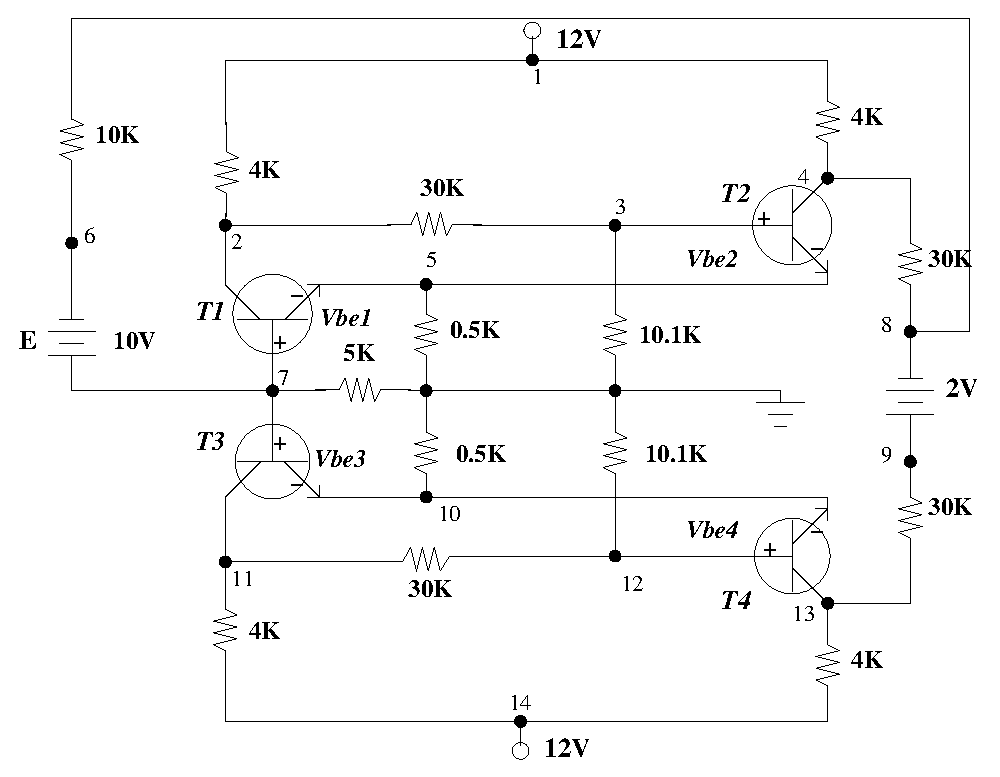
\includegraphics[scale=0.4]{fig/newchua.eps}
\caption{Chua's circuit.}
\label{newchua}
\end{figure}


The resulting equation system is:

{\tiny
\begin{equation}
\begin{array}{l}
f_1=4.3663V_{be2}+0.6103168 \times 10^{-5} e^{(40V_{be1})}-12 + \\ 0.2863168\times 10^{-5}e^{(40V_{be2})}=0 \\ \\
f_2=5.4V_{be1}+V_{be3}+0.3580\times 10^{-5}e^{(40V_{be1})}-22 + \\7\times 10^{-7}e^{(40V_{be3})}+  5\times 10^{-7}e^{(40V_{be4})}+0.6620\times 10^{-5}e^{(40V_{be2})}=0 \\ \\
f_3=4.3663V_{be4}+0.6103168\times 10^{-5}e^{(40V_{be3})}-12 + \\0.2863168\times 10^{-5}e^{(40V_{be4})}=0 \\
%f_1=4.3663v_2+0.6103168 \times 10^{-5} e^{(40v_1)}-12 +0.2863168\times 10^{-5}e^{(40v_2)}=0 \\ \\
%f_2=5.4v_1+v_3+0.3580\times 10^{-5}e^{(40v_1)}-22 +7\times 10^{-7}e^{(40v_3)}+  5\times 10^{-7}e^{(40v_4)}+0.6620\times 10^{-5}e^{(40v_2)}=0 \\ \\
%f_3=4.3663v_4+0.6103168\times 10^{-5}e^{(40v_3)}-12 +0.2863168\times 10^{-5}e^{(40v_4)}=0 \\
\end{array}
\end{equation}
}

Now, the DBH is applied to solve the circuit by using the next parameters: $a=1$, $C=1$, a value of $\pm 5.2$
for initial and final point of each voltage base to emiter $V_{be}$ and the initial point for the Homotopy path is selected as $A=[V_{be1}=-5.2,V_{be2}=-5.2,V_{be3}=-5.2,V_{be4}=-5.2]$.

Equilibrium equation is the same as employed in \cite{homo_chua}. The variables to be solved are branch voltages: $V_{be1}$, $V_{be2}$, $V_{be3}$ and $V_{be4}$. Figure \ref{chuaf} shows the Homotopy path for branch voltage $V_{be1}$. The final point for the path was $B=[V_{be1}=-5.2,V_{be2}=-5.2,V_{be3}=5.2,V_{be4}=-5.2]$. Finally, Homotopy was able to locate all the 9 solutions in just one path. This result is interesting considering that in recent works \cite{homo_yamamura}\cite{homo_jaewook} (applied to the same circuit) only one solution was found or some solutions were found by selecting (random or arbitrary) different initial points, that is, different and unconnected Homotopy paths.

\begin{figure}[hbtp]
\centering
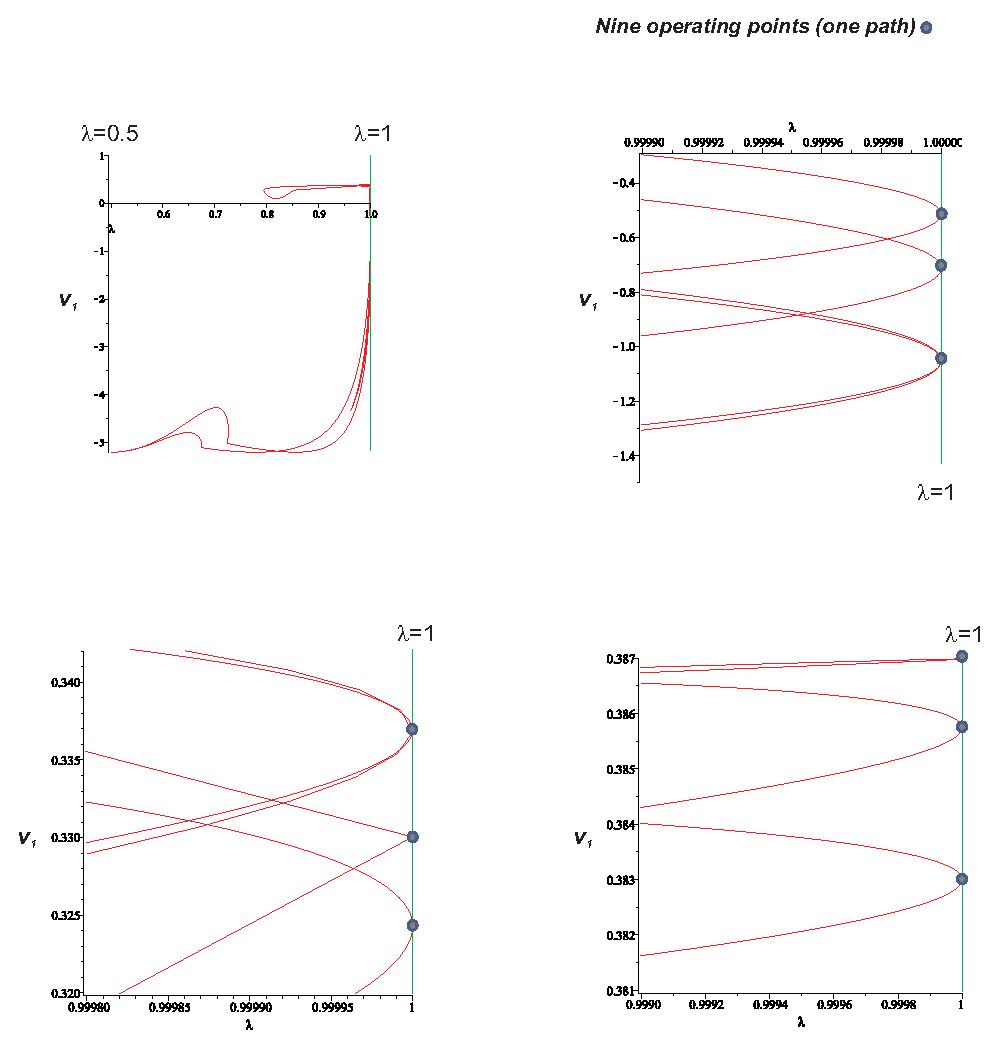
\includegraphics[scale=0.5]{fig/chuanew.eps}
\caption{Solutions for Chua's circuit.}
\label{chuaf}
\end{figure}



\section{Conclusions}

A new kind of Homotopy was presented, it is named double bounded algebraic Homotopy, which contains just 2 solution lines. It was demonstrated the symmetry of the Homotopy paths. 
Additionally, it was illustrated the use of Homotopy in a benchmark circuital case, showing its potential to be employed in analysis of non-linear circuits.

\bibliographystyle{amsplain}
\bibliography{carta2}

\end{document}
